
\begin{SCfigure*}
	\centering
	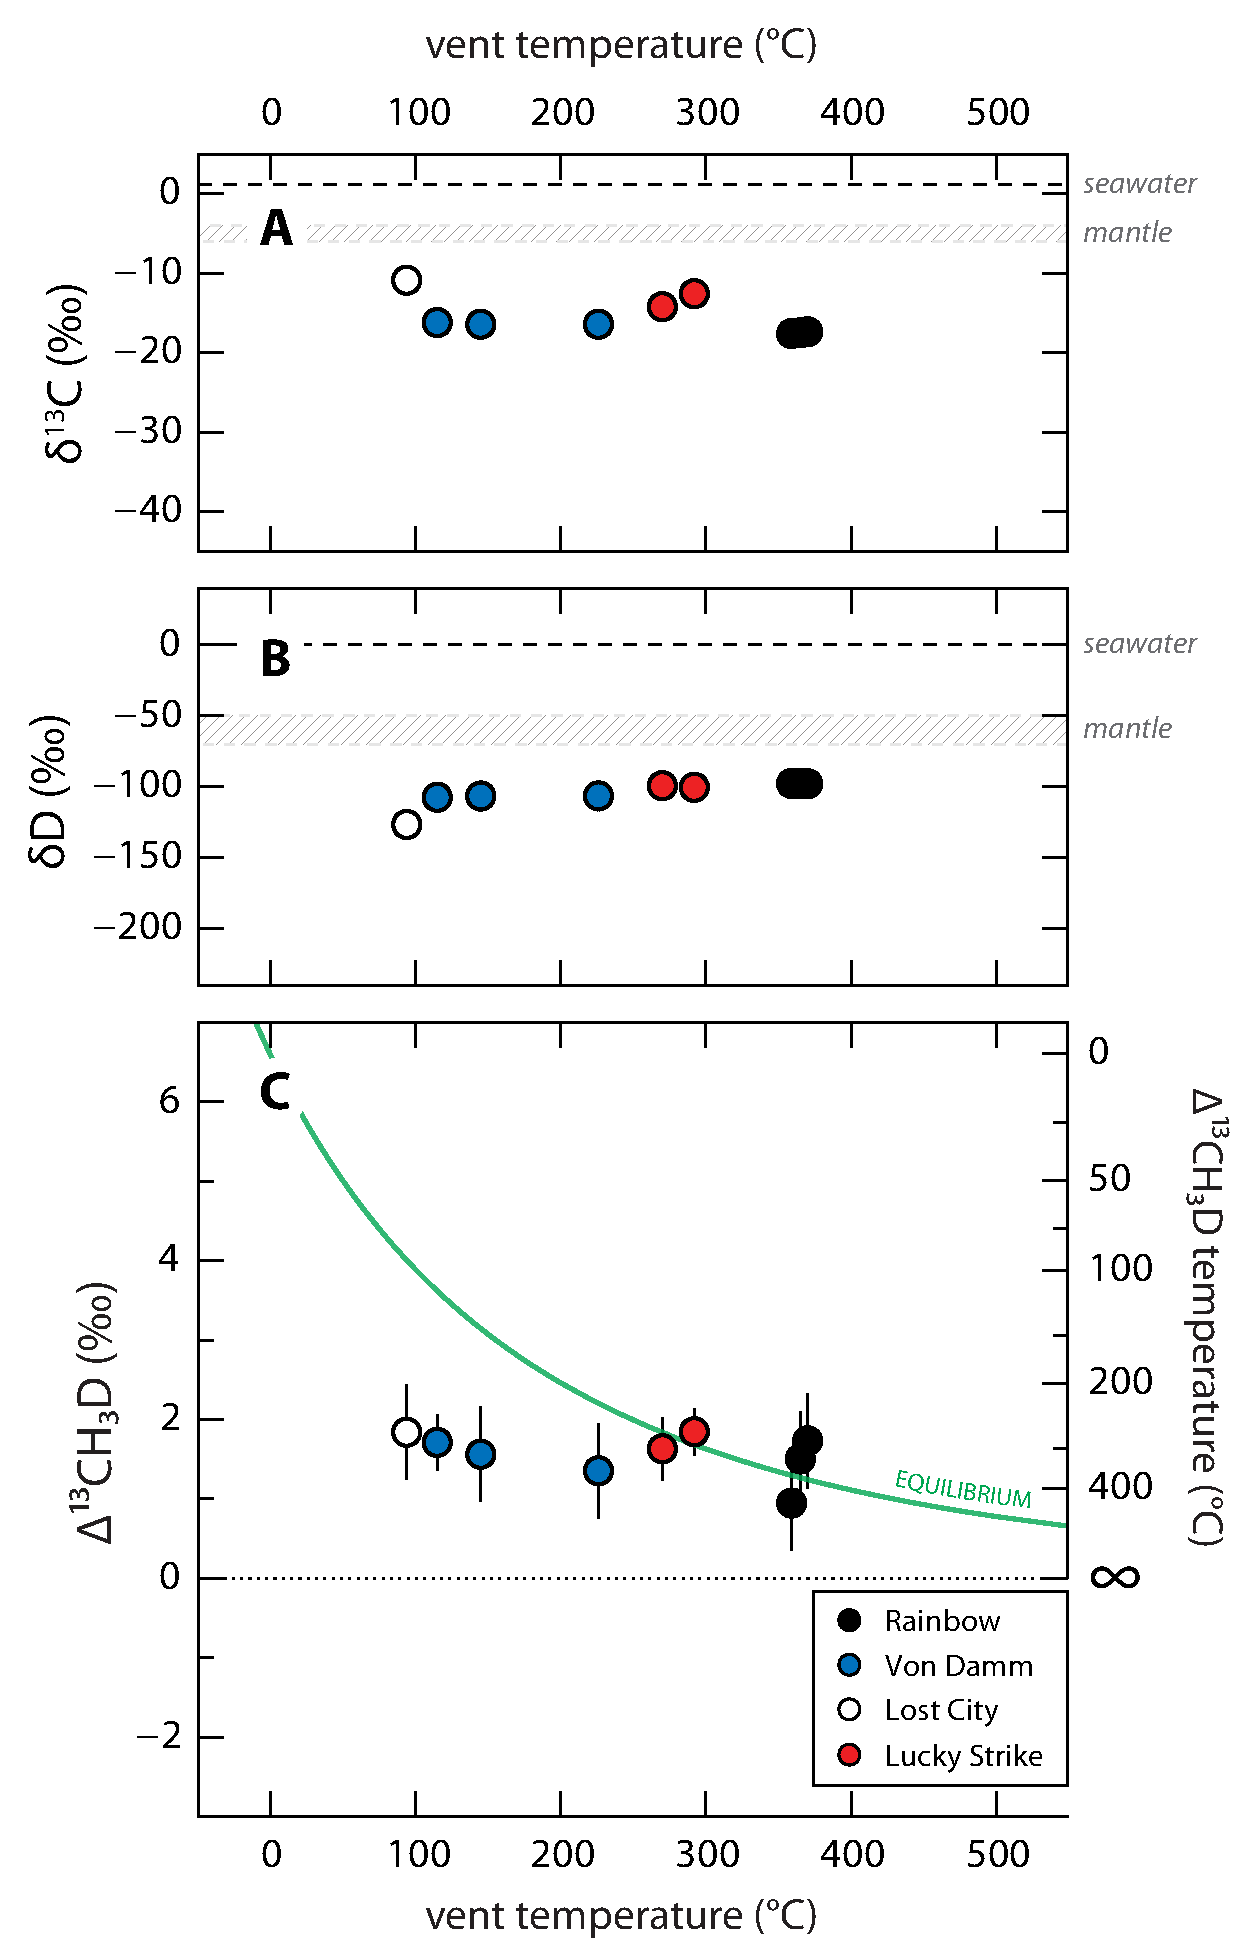
\includegraphics[width=0.6\linewidth]{figures/Fig3.1}
	\caption[Isotope and isotopologue ratios of methane at studied vent sites]{%
		Comparison of (\textbf{A}) δ\textsuperscript{13}C, (\textbf{B}) δD, and
		(\textbf{C}) Δ\textsuperscript{13}CH\textsubscript{3}D values of methane
		across vent sites. Data and error bars (95\% confidence interval) are
		from \autoref{tab:3:1}. In all panels, points are plotted against measured vent
		temperature (\autoref{tab:3:2}). The isotopic compositions of inorganic carbon (A)
		and hydrogen (B) in seawater and in the mantle are shown \parencite{Javoy++_1986_CG,Blank++_1993_GCA,Clog++_2013_EPSL}. In (C), the green line
		represents the clumped isotopologue composition at equilibrium. The
		Δ\textsuperscript{13}CH\textsubscript{3}D temperature scale corresponds
		to the calibration from \textcite{Wang++_2015_S}.
	}
	\label{fig:3:1}
\end{SCfigure*}
